\section{Auswertung}
\label{sec:Auswertung}

In der folgenden Auswertung wird die Filterkurve des Selektiv-Verstärkers untersucht
und mithilfe einer Brückenschaltung die Suszeptibilitäten verschiedener Selten-Erd-Metalle bestimmt,
sowie mit den theoretisch ermittelten Suszeptibilitäten verglichen.


\subsection{Theoretische Bestimmung der Suszeptibilität}

Zum Vergleich der zu bestimmenden Suszeptibilitäten werden diese zunächst theoretisch mithilfe der Hundschen Regeln in \autoref{sec:Theorie} ermittelt.
Bei den hier verwendeten Selten-Erd-Metallen handelt es sich um $\ce{Dy2O3}$, $\ce{Gd2O3}$ und $\ce{Nd2O3}$.
Bei allen Stoffen ist die maximale Hauptquantenzahl $n = 4$, woraus für die Orientierungsquantenzahl $m =$ (-3, -2, -1, 0, 1, 2, 3) ergibt. 
Damit folgt für die drei Stoffe:

\begin{itemize}
  \item $\ce{Dy2O3}$ besitzt neun Elektronen in der 4f-Schale und damit mehr als die Anzahl von $m$, weswegen zwei Elektronen einen negativen Spin haben.
        Damit ist $ S = \sum_{i} s_i = \frac{5}{2}$ und der Drehimpuls ergibt sich zu $L = \sum_i m_i = 5$.
        Da die Schale mehr als halb voll ist, ist der Gesamtdrehimpuls $J = L + S = 5 + \frac{5}{2} = 7,5$.
        Nach \autoref{eq:lande} ist der Landé-Faktor somit $g_\text{j} = \frac{4}{3}$.

  \item $\ce{Gd2O3}$ besitzt sieben Elektronen in der 4f-Schale mit dem selben Spin folgt für $S = \frac{7}{2}$ und für $L = 0$, da $m$ gleich der Anzahl an Elektronen ist.
        Damit ist $J = S = 3.5$ und $g_\text{j} = 2$

  \item $\ce{Nd2O3}$ besitzt drei Elektronen in der 4f-Schale, also ist $S = \frac{3}{2}$ und $L = 6$.
        Aufgrund der weniger als halbvollen Schale folgt für $J = L - S = 6 + \frac{3}{2} = 4,5$ und für $g_\text{j} = \frac{8}{11}$
\end{itemize}

Für die Anzahl der Momente pro Volumen gilt
\begin{equation}
  N = 2 \, N_\text{a} \, \frac{\rho}{M_\text{mol}} \, ,
\end{equation}
mit der Avogadrokonstante $N_\text{a} = \qty{6.02214076e23}{\per\mol}$, der Dichte $\rho$ und der molaren Masse $M_\text{mol}$.

Diese Werte und die berechnete Anzahl der Momente pro Volumen sind in \autoref{tab:momente} dargestellt.
\begin{table}
  \centering
  \caption{Die Werte zur Berechnung der Anzahl der Momente $N$ mit den Dichten $\rho$ nach \cite{v606}.}
  \label{tab:momente}
  \begin{tabular}{c c c c}
    \toprule
    Stoff &     
    $\rho_\text{w} \mathbin{/} \unit[per-mode=reciprocal]{\gram\per\cubic\centi\meter}$ & 
    $M_\text{mol} \mathbin{/} \unit[per-mode=reciprocal]{\gram\per\mol}$ & 
    $N \mathbin{/} \unit[per-mode=reciprocal]{\per\cubic\centi\meter} \cdot 10^{22}$ \\ 
    \midrule
    Dy2O3 &         7,80 &       373,00 &            2,518643 \\
    Gd2O3 &         7,40 &       362,50 &            2,405534 \\
    Nd2O3 &         7,24 &       336,48 &            2,591554 \\
    \bottomrule
    \end{tabular}
\end{table}

Daraus kann nach \autoref{eq:susz_theo} die theoretische Suszeptibilität der Stoffe in \autoref{tab:susz_theo} berechnet werden.
\begin{table}
  \centering
  \caption{Die theoretisch berechneten Suszeptibilitäten der drei Stoffe.}
  \label{tab:susz_theo}
  \begin{tabular}{ c c}
    \toprule
    Stoff & 
    $\chi_\text{theoretisch}$ \\
    \midrule
    $\ce{Dy2O3}$ &  0,025421 \\
    $\ce{Gd2O3}$ &  0,013497 \\
    $\ce{Nd2O3}$ &  0,003021 \\
    \bottomrule
  \end{tabular}
\end{table}


\subsection{Bestimmung der Filterfrequenz und Güte des Selektivverstärkers}

Unter Verwendung eines Selektiv-Verstärkers mit einer Güte von $\text{Q} = 20$
und einer konstanten Sinus-Speisespannung von $U_\text{Sp} = \qty{35}{kHz}$ 
werden für Frequenzen im Bereich $20 - \qty{40}{kHz}$ die
Ausgangsspannungen $U_\text{A}$ untersucht.
Die Messdaten sind in \autoref{tab:spannung} zu sehen.
\begin{table}[H]
  \centering
  \caption{Die Messdaten der Ausgangsspannungen des Selektiv-Verstärkers.}
  \label{tab:spannung}
  \begin{tabular}{c c}
    \toprule
    $\nu \mathbin{/} \unit{kHz}$ & $U_\text{A} \mathbin{/} \unit{V}$ \\
    \midrule
      20,0 & 0,085 \\
      22,5 & 0,110 \\
      25,0 & 0,150 \\
      27,0 & 0,190 \\
      30,0 & 0,310 \\
      32,8 & 0,800 \\
      33,3 & 1,200 \\
      34,1 & 1,900 \\
      35,4 & 2,000 \\
      36,0 & 1,600 \\
      36,9 & 0,840 \\
      38,3 & 0,530 \\
      39,3 & 0,410 \\
    \bottomrule
  \end{tabular}
\end{table}

Zur Bestimmung der Filterfrequenz $\nu_\text{0}$ sowie der maximalen Ausgangsspannung $U_\text{A}$ 
werden die Messdaten unter Betrachtung einer Gaußverteilung wie folgt angenähert:
\begin{equation}\label{eq:gauss}
  U_\text{g}(\nu) = a \cdot \exp\left( -\frac{(\nu-\nu_\text{0})^2}{b} \right) \, .
\end{equation}
Die Messdaten und die daraus berechnete Ausgleichsfunktion wird in \autoref{fig:plot1} dargestellt.
\begin{figure}
  \centering
  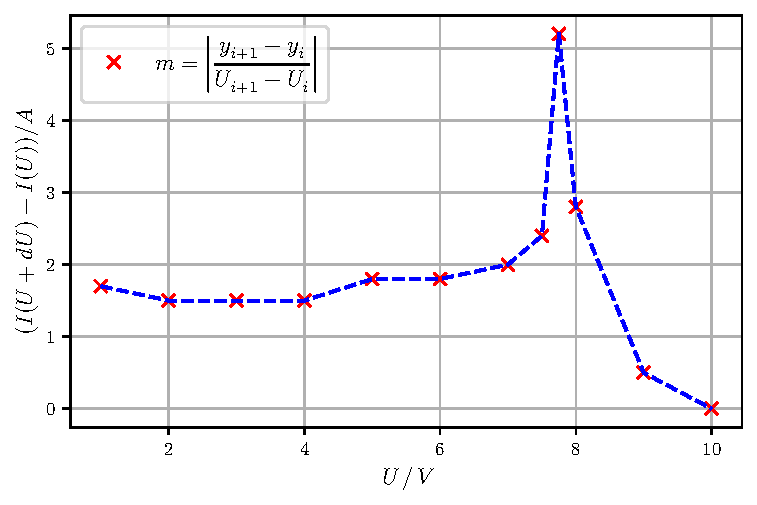
\includegraphics[width=0.8\linewidth]{plot1.pdf}
  \caption{Die Messdaten sowie die Ausgleichsrechnung nach Gaußverteilung der Spannung in Abhängigkeit der Frequenz.}
  \label{fig:plot1}
\end{figure}
Aus \autoref{eq:gauss} ergeben sich die Parameter
\begin{align*}
  a &= \qty{1.98(15)}{\volt} \, ,\\
  b &= \num{6.1(1.2)} 
\end{align*}
und die zu bestimmenden Werte
\begin{align*}
  \nu_\text{0} = \qty{34.95(14)}{kHz} \approx \qty{35}{kHz} &\quad 
  \text{mit} \quad U_\text{A} = \qty{1.97}{\volt} \approx \qty{2}{\volt} \, .
\end{align*}

Zur Bestimmung der Güte werden zusätzlich noch diejenigen Frequenzen $\nu_{-}$ und $\nu_{+}$ in \autoref{fig:plot1} erfasst,
bei denen das Verhältnis von Aus- und Eingangsspannung $\text{U}_{A} / \text{U}_{E}$ auf $1/\sqrt{2}$ absingt.
Diese ergeben sich zu
\begin{align*}
  \nu_{-} = \qty{33.52(14)}{kHz} \quad \text{und} \quad \qty{36.38(14)}{kHz} \, .
\end{align*}
Die experimentell ermittelte Güte des Selektivverstärkers ist somit
\begin{equation}
  Q = \frac{\nu_0}{\nu_{+} - \nu_{-}} = (\num{12(0.8)}) \, .
\end{equation}


\subsection{Experimentelle Bestimmung der Suszeptibilität}

Für die folgende experimentelle Untersuchung der Suszeptibilität wird eine Sinusspannung 
mit der davor bestimmten Frequenz von $\qty{35}{kHz}$ und einer Speisespannung von $U_\text{Sp} = \qty{1}{\volt}$ verwendet.
Da jede Probe in Pulverform vorliegt, ist die Dichte $\rho_\text{P}$ geringer als die eines Einkristalls.
Der real Querschnitt der Probe ergibt sich also zu
\begin{equation}
  Q_\text{real} = \frac{M_\text{P}}{l \, \rho_\text{w}} \, ,
\end{equation}
dabei ist $M_\text{P}$ die Masse der Probe, $l$ die Länge der Probe und $\rho_\text{w}$ die Dichte eines Einkristalls.

In \autoref{tab:proben} sind die Werte der Proben dargestellt.
\begin{table}
  \centering
  \caption{Die Kennwerte der jeweiligen Stoffproben.}
  \label{tab:proben}
  \begin{tabular}{c c c c c}
    \toprule
    Stoff &   
    $m \mathbin{/} \mathrm{g}$ &
    $l \mathbin{/} \mathrm{cm}$ &
    $\rho_\text{w} \mathbin{/} \unit[per-mode=reciprocal]{\gram\per\cubic\centi\meter}$ & 
    $Q_\text{real} \mathbin{/} \unit{\centi\meter\squared}$ \\
    \midrule
    $\ce{Dy2O3}$ & 15,10 &  15,9 & 7,80 & 0,1217 \\
    $\ce{Gd2O3}$ & 14,08 &  16,5 & 7,40 & 0,1153 \\
    $\ce{Nd2O3}$ &  8,48 &  16,5 & 7,24 & 0,0709 \\
    \bottomrule
  \end{tabular}
\end{table}

In den folgenden Tabellen sind die Messdaten der Stoffproben dargestellt, 
dabei werden die Brückenspannungen und Widerstände vor und nach Einführen der Proben mithilfe ihrer Differenz verglichen.
\begin{table}[H]
  \centering
  \caption{Die Messdaten für $\ce{Dy2O3}$.}
  \label{tab:dy}
  \begin{tabular}{c c c c c c}
    \toprule 
    
    \multicolumn{1}{c}{$U_\text{v} \mathbin{/} \unit{\milli\volt}$} &
    \multicolumn{1}{c}{$R_\text{v} \mathbin{/} \unit{\ohm} $} &
    \multicolumn{1}{c}{$U_\text{n} \mathbin{/} \unit{\milli\volt}$} &
    \multicolumn{1}{c}{$R_\text{n} \mathbin{/} \unit{\ohm}$}& 
    \multicolumn{1}{c}{$\increment U \mathbin{/} \unit{\milli\volt}$}&
    \multicolumn{1}{c}{$\increment R \mathbin{/} \unit{\ohm}$} \\

    \cmidrule(lr){1-2} \cmidrule(lr){3-4} \cmidrule(lr){5-6}

    5,5 & 3,405 & 0,40 & 1,855 &    5,10 &   1,550 \\
    5,6 & 3,330 & 0,33 & 1,825 &    5,27 &   1,505 \\
    5,4 & 3,330 & 0,31 & 1,830 &    5,09 &   1,500 \\
    \bottomrule
  \end{tabular} 
\end{table}

\begin{table}[H]
  \centering
  \caption{Die Messdaten für $\ce{Gd2O3}$.}
  \label{tab:gd}
  \begin{tabular}{c c c c c c}
    \toprule 
    
    \multicolumn{1}{c}{$U_\text{v} \mathbin{/} \unit{\milli\volt}$} &
    \multicolumn{1}{c}{$R_\text{v} \mathbin{/} \unit{\ohm} $} &
    \multicolumn{1}{c}{$U_\text{n} \mathbin{/} \unit{\milli\volt}$} &
    \multicolumn{1}{c}{$R_\text{n} \mathbin{/} \unit{\ohm}$}& 
    \multicolumn{1}{c}{$\increment U \mathbin{/} \unit{\milli\volt}$}&
    \multicolumn{1}{c}{$\increment R \mathbin{/} \unit{\ohm}$} \\

    \cmidrule(lr){1-2} \cmidrule(lr){3-4} \cmidrule(lr){5-6}

    2,5 & 3,370 & 0,29 & 2,69 &    2,21 &   0,680 \\
    2,8 & 3,355 & 0,28 & 2,64 &    2,52 &   0,715 \\
    2,7 & 3,370 & 0,26 & 2,68 &    2,44 &   0,690 \\    
    \bottomrule
  \end{tabular} 
\end{table}

\begin{table}[H]
  \centering
  \caption{Die Messdaten für $\ce{Nd2O3}$.}
  \label{tab:nd}
  \begin{tabular}{c c c c c c}
    \toprule 
    
    \multicolumn{1}{c}{$U_\text{v} \mathbin{/} \unit{\milli\volt}$} &
    \multicolumn{1}{c}{$R_\text{v} \mathbin{/} \unit{\ohm} $} &
    \multicolumn{1}{c}{$U_\text{n} \mathbin{/} \unit{\milli\volt}$} &
    \multicolumn{1}{c}{$R_\text{n} \mathbin{/} \unit{\ohm}$}& 
    \multicolumn{1}{c}{$\increment U \mathbin{/} \unit{\milli\volt}$}&
    \multicolumn{1}{c}{$\increment R \mathbin{/} \unit{\ohm}$} \\

    \cmidrule(lr){1-2} \cmidrule(lr){3-4} \cmidrule(lr){5-6}

    0,440 & 3,340 & 0,38 & 3,305 &   0,060 &   0,035 \\
    0,425 & 3,380 & 0,36 & 3,285 &   0,065 &   0,095 \\
    0,510 & 3,405 & 0,34 & 3,315 &   0,170 &   0,090 \\
    \bottomrule
  \end{tabular} 
\end{table}

Die Suszeptibilität $\chi$ lässt sich dadurch nach \autoref{eq:delU} und \autoref{eq:delR} zu den Werten in \autoref{tab:susz_alle} berechnen
und mit den theoretischen aus \autoref{tab:susz_theo} vergleichen.
\begin{table}
  \centering
  \caption{Die experimentell und theoretisch bestimmten Suszeptibilitäten.}
  \label{tab:susz_alle}
  \begin{tabular}{c c c c}
    \toprule
    Stoff &    
    $\chi_\text{U}$ &
    $\chi_\text{R}$ &
    $\chi_\text{theoretisch}$ \\
    \midrule
    $\ce{Dy2O3}$ & 0,146616 & 0,021642 &   0,025421 \\
    $\ce{Gd2O3}$ & 0,071794 & 0,010460 &   0,013497 \\
    $\ce{Nd2O3}$ & 0,004798 & 0,001793 &   0,003021 \\
    \bottomrule
  \end{tabular}
\end{table}